\documentclass[12pt]{article}
\usepackage[utf8]{inputenc}
\usepackage{parskip}
\usepackage[spanish]{babel}
\usepackage{amsmath, amssymb}
\usepackage{graphicx}
\usepackage{makecell}
\usepackage{geometry}
\usepackage{caption}
\usepackage{float}
\usepackage[hidelinks]{hyperref}


% --------------------- Comandos para pie de página ---------------------
\usepackage[backend=biber, style=apa]{biblatex}
\addbibresource{referencias.bib}
\usepackage{hyperref}
\usepackage{url}
\usepackage{csquotes}

\makeatletter
\g@addto@macro{\UrlBreaks}{\UrlOrds}
\makeatother

\renewcommand{\footnoterule}{%
  \kern -3pt                         % Espacio vertical sobre la línea
  \hrule width \textwidth height 0.4pt % Ancho total de la página y grosor
  \kern 2.6pt                        % Espacio vertical debajo de la línea
}
% -----------------------------------------------------------------------

\addbibresource{referencias.bib}
\geometry{letterpaper, margin=2.5cm}
\setlength{\parskip}{1em}

\begin{document}
\begin{titlepage}
\begin{center}
    % Logos
    \begin{minipage}{0.3\textwidth}
        
\includegraphics[width=0.8\linewidth]{imagenes/UNAM_Logo.png}
    \end{minipage}\hfill
    \begin{minipage}{0.4\textwidth}
        \begin{center}
            \textbf{\Large Universidad Nacional Autónoma de México}\\[0.2cm]
            \textbf{Facultad de Ciencias}\\[0.2cm]
        \textbf{Bases de Datos}
        \end{center}
    \end{minipage}\hfill
    \begin{minipage}{0.3\textwidth}
        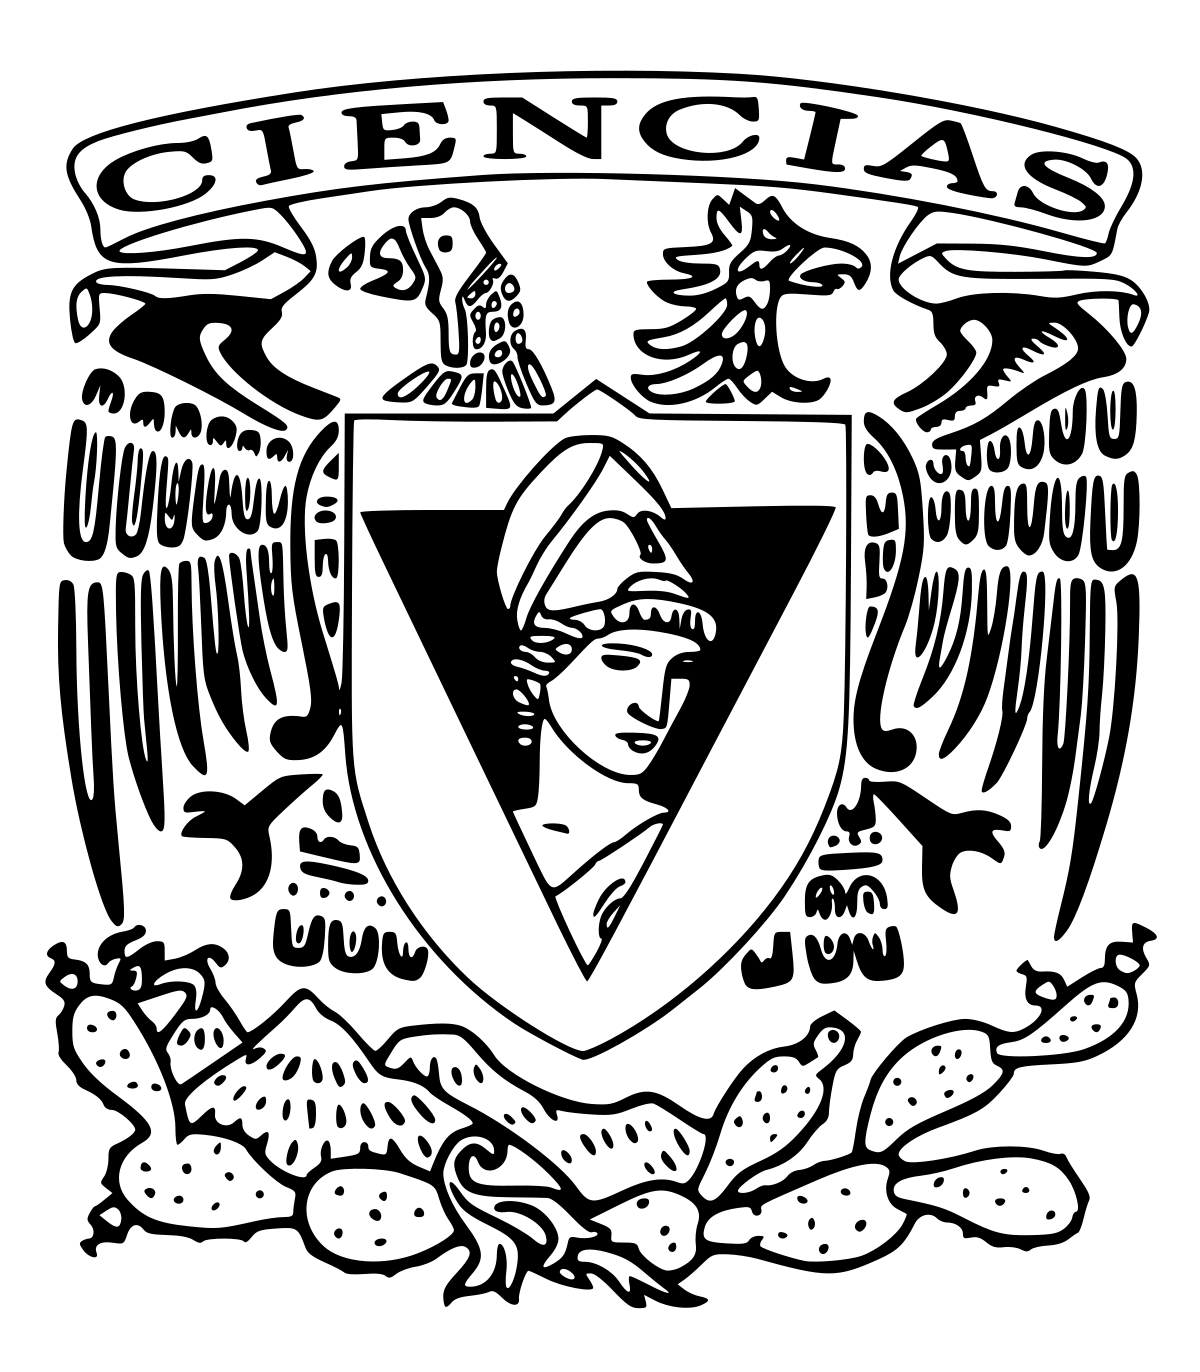
\includegraphics[width=0.8\linewidth]{imagenes/Logo_FC.png}
    \end{minipage}
    \vspace{3cm}
    \textbf{\large Tarea 3}\\
    Licenciatura en Ciencias de la Computación\\
    Profesor: Gerardo Avilés Rosas \\
    \vspace{2cm}
    \textbf{Integrantes: }\\
    Cisneros Tenorio Diego Alexander\\
    Nuñez Ruiz José Manuel \\
    Olmos Ortiz Andrea Lucia\\
    Reynoso Ascencio Alexa \\
    Vega Navas Saúl \\
    \vspace{2cm}
    \textbf{Fecha de entrega: } 9 de Octubre del 2026
    \vfill
\end{center}
\end{titlepage}
\tableofcontents
\newpage

% Preguntas

 \section{Preguntas de repaso}
\subsection*{i. }
\addcontentsline{toc}{subsection}{i.}

\textbf{¿Qué es una relación y qué características tiene?}

Una relación $R$ sobre los conjuntos de entidades $A_1, A_2, A_3, \dots, A_n$ es un subconjunto del producto cartesiano de los mismos: $R \subseteq A_1 \times A_2 \times A_3 \times \dots \times A_n$. En las bases de datos relacionales se representa mediante una estructura de tabla compuesta por un nombre único, un conjunto fijo de atributos (columnas) y un conjunto de tuplas (filas).

Las características de una relación en el Modelo Relacional se dividen en las siguientes:

\begin{itemize}
    \item \textbf{Dominio:} Conjunto finito de valores homogéneos y atómicos caracterizados por un nombre específico.
    \item \textbf{Atributos:} Elemento que participa en la descripción de las entidades y constituye una pieza específica de información para un determinado dominio. Cada atributo (columna) debe poseer un nombre único en la relación, y absolutamente todos los atributos deben contener valores atómicos.
    \item \textbf{Llaves:} Conjunto no vacío de atributos que identifican de manera unívoca y mínima cada tupla. Estas se subdividen rigurosamente en:
    \begin{itemize}
        \item \textit{Llave primaria:} Permite identificar las tuplas de la relación de forma única.
        \item \textit{Llaves candidatas:} Atributos que poseen la capacidad de identificar de manera única a una tupla, pero que no fueron seleccionados como llave primaria.
        \item \textit{Llave foránea:} Conjunto no vacío de atributos cuyos valores obligatoriamente deben de coincidir con los valores de la llave primaria en otra relación.
    \end{itemize}
    \item \textbf{Restricciones:} Consisten en estructuras no permitidas dentro del modelo, dividiéndose en dos clasificaciones principales: inherentes y del usuario.
    \item \textbf{Propiedades de las Relaciones:} Toda relación debe contar con un nombre único. En la intersección exacta de una columna y una fila siempre se encontrará un único valor, por lo que no se permiten bajo ninguna circunstancia los atributos multivaluados.
    \item \textbf{Unicidad y Disposición de Tuplas:} No se admite la existencia de tuplas duplicadas, garantizando que cada renglón sea irrepetible. Además, es completamente irrelevante el orden en el que se presenten las tuplas.
    \item \textbf{Disposición de Atributos:} Los atributos se encuentran desordenados; el orden lógico o físico de las columnas no altera la estructura. Por ejemplo, la relación \texttt{alumno(nombre, num\_cta, edad)} es equivalente a \texttt{alumno(num\_cta, nombre, edad)}.
\end{itemize}

 \subsection*{ii. }

\addcontentsline{toc}{subsection}{ii.}
\textbf{¿Qué es un esquema de relación?}\\ \\
Un esquema de relación es la descripción formal de la estructura de una relación. Está definido por un nombre, un conjunto de atributos y un dominio asociado a cada atributo. \\ \\
Permite abstraer los datos concretos almacenados en una tabla, estableciendo su estructura y las restricciones que deben cumplir sus datos. Se puede representar conserva la notación matemática $(R(A_1,A_2,\ldots,A_n))$, donde $(R)$ es el nombre de la relación y $(A_1,A_2,\ldots,A_n)$ son sus atributos.
 \subsection*{iii.}

\addcontentsline{toc}{subsection}{iii.}

\textbf{¿Qué es una llave primaria?, ¿qué es una llave candidata?, ¿qué es una llave mínima?, ¿qué es una
super llave?}

\begin{itemize}
    \item \textbf{Llave primaria:} Es una llave candidata elegida como el medio principal para identificar tuplas dentro de una relación.
    \item \textbf{Llave candidata:} Es una super llave es un subconjunto del conjunto de atributos de la relación, a la cual no se le puede eliminar ningún atributo sin perder la capacidad de identificar de forma única a cada tupla.
    \item \textbf{Llave mínima:} Es una super llave para las cuales ningún subconjunto propio es una superllave.
    \item  \textbf{Super llave:} Conjunto de uno o más atributos cuyos valores no se repiten en tuplas distintas de la relación, los cuales permiten identificar de manera única una tupla en la relación.
\end{itemize}
 \section*{iv.}
\subsection*{Restricciones de la Llave Primaria (PK)}
\begin{itemize}
    \item \textbf{Integridad de Entidad (NOT NULL):} Ninguna columna de la PK puede contener valores nulos, sino que debe contar obligatoriamente con una identificación válida.

    \item \textbf{Unicidad (UNIQUE):} La tupla que constituye a la PK debe ser distinta de las demás dentro de la relación, evitando la duplicidad de entidades y permitiendo identificar a cada entidad como única.
\end{itemize}

\subsection*{Restricciones de la Llave Foránea (Foreign Key)}

\begin{itemize}
    \item \textbf{Integridad Referencial:} Todo valor almacenado en la columna de la llave foránea debe existir previamente como PK de la tabla a la que se hace referencia, lo que restringe las inserciones o actualizaciones de un registro a la existencia de dicho valor (\textbf{Restricción de Inserción o Modificación en la Tabla Hija}) a menos que el campo permita explícitamente valores nulos.
    \item \textbf{Restricción de Modificación o Eliminación en la Tabla Padre:} Impide la escenarios de "registros huérfanos" mediante la aplicación de normas sobre la primaria referenciada:
    \begin{itemize}
        \item \textbf{RESTRICT / NO ACTION:}Un registro en la tabla padre no puede ser modificado o eliminado si existen registros en la tabla hija que dependen de éste.
        \item \textbf{CASCADE:} Elimina o actualiza automáticamente los registros correspondientes en la tabla hija si el registro padre es modificado o eliminado.
        \item \textbf{SET NULL:} Asigna el valor NULL a la llave foránea en la tabla hija si el registro padre es eliminado o modificado (si es que la columna permite nulos).
        \item \textbf{SET DEFAULT:} Asigna un valor por defecto en la tabla hija cuando el registro padre se elimina o modifica.
    \end{itemize}
\end{itemize}

 \subsection*{V. }

\addcontentsline{toc}{subsection}{V.}
    
\textbf{Investiga que cuáles son las Reglas de Codd y explica con tus propias palabras cada una de ellas. Indica por qué consideras que son importantes.}

Las reglas de Codd son un conjunto de requerimientos necesarios para construir un SMBD apto para implementar el modelo relacional. Son un conjunto de 13 reglas (0-12), a continuación se explicará el contenido de cada regla:
\begin{enumerate}[start=0]
    \item \textit{Cualquier sistema que se anuncie o se afirme que es un sistema de gestión de bases de datos relacionales debe ser capaz de gestionar bases de datos íntegramente a través de sus capacidades
    relacionales} \cite{Codd1985}

    Esta regla indica que un SMBD relacional debe ejecutar cualquier acción dentro del sistema mediante operaciones con tablas, administrándose a sí mismo mediante dichas operaciones.    
        
    \item \textit{Toda la información de una base de datos relacional se representa de forma explícita en el nivel lógico y de una única manera: mediante valores en tablas.}\cite{Codd1985}

    Indica que cualquier dato que el sistema almacene, incluyendo al catálogo de datos, debe hacerlo únicamente mediante el uso de tablas.
    
    \item \textit{Se garantiza que se puede acceder lógicamente a todos y cada uno de los datos (valores atómicos) de una base de datos relacional mediante una combinación del nombre de la tabla, el valor de la clave primaria y el nombre de la columna}\cite{Codd1985}
    
    Significa que por cada dato almacenado en el sistema, debe existir al menos una forma de acceder a él, mediante información sobre su ubicación, como el nombre de la tabla a la que pertenece, la fila (identificada por la llave primaria) y la columna en que se ubica.
    
    \item \textit{Los valores nulos (distintos de la cadena de caracteres vacía o de una cadena de caracteres en blanco, y distintos del cero o de cualquier otro número) son admitidos en los SGBD plenamente relacionales para representar, de forma sistemática e independiente del tipo de datos, la información que falta y la información no aplicable.}\cite{Codd1985}

    Esta regla indica que el sistema debe ser capaz de representar a los valores nulos de forma universal, independientemente de la tabla en la que falta la información. Esta regla resulta útil al momento de implementar restricciones en las que algunos datos no pueden ser nulos (Como las llaves), garantizando la integridad de los datos.
    
    \item \textit{La descripción de la base de datos se representa a nivel lógico de la misma manera que los datos ordinarios, de modo que los usuarios autorizados puedan aplicar el mismo lenguaje relacional a su consulta que el que aplican a los datos normales.}\cite{Codd1985}
    
    Significa que la descripción sobre el propio sistema, el catálogo de datos (tablas y columnas), debe representarse dentro del sistema mediante tablas, como si fuera otro dato más con el que se puede interactuar.
    
    \item \textit{Un sistema relacional puede admitir varios lenguajes y diversos modos de uso de terminales (por ejemplo, el modelo de «rellenar los espacios en blanco»). Sin embargo, debe existir al menos un lenguaje cuyas sentencias puedan expresarse, según una sintaxis bien definida, como cadenas de caracteres y que sea exhaustivo a la hora de admitir todos los elementos siguientes:
    Definición de datos, definición de vistas, manipulación de datos (interactiva y mediante programa), restricciones de integridad,  autorización, límites de las transacciones (inicio, confirmación y reversión).} \cite{Codd1985}
    
    Esta regla implica que, aunque el sistema pueda ofrecer múltiples interfaces o lenguajes de apoyo para los usuarios, debe existir al menos un lenguaje principal y bien definido, capaz de gestionar todos los aspectos de la base de datos.
    
    \item \textit{Todas las vistas que son teóricamente actualizables también lo son por el sistema.}\cite{Codd1985}

    Significa que, si es posible modificar un dato desde una de las vistas sin ambigüedades, entonces el sistema debe permitir realizar dicha operación y reflejar el cambio automáticamente en las tablas correspondientes.

    \item \textit{La capacidad de tratar una relación base o una relación derivada como un único operando se aplica no solo a la recuperación de datos, sino también a la inserción, actualización y eliminación de datos}\cite{Codd1985}
    
    Indica que el sistema debe ser capaz de operar con conjuntos de datos para consultar, insertar, modificar y eliminar datos. Esta propiedad permite que los SMBD sean capaces de manipular grandes cantidades de datos de forma eficiente.
    
    \item \textit{Los programas de aplicación y las actividades de los terminales no se ven afectados lógicamente cuando se producen cambios, ya sea en las representaciones de almacenamiento o en los métodos de acceso.} \cite{Codd1985}

    Esta regla hace referencia a que los SMBD deben garantizar la independencia física, es decir que cualquier modificación en la forma de almacenamiento y el acceso a los datos, no debe afectar a las aplicaciones.
    
    \item \textit{Los programas de aplicación y las actividades de los terminales no se ven afectados lógicamente cuando se realizan cambios en las tablas base.}\cite{Codd1985}
    
    Implica que el SMBD debe garantizar la independencia lógica, es decir que al realizar modificaciones sobre las tablas para reestructurarlas, no se debe afectar a las aplicaciones o programas que usen la base de datos para funcionar.
    
    \item \textit{Las restricciones de integridad específicas de una base de datos relacional concreta deben poder definirse en el sublenguaje de datos relacionales y almacenarse en el catálogo, no en los programas de aplicación}   \cite{Codd1985}
    
    Implica que cualquier regla de integridad, como la integridad referencial o la integridad de entidad, debe almacenarse directamente en la base de datos como un dato más. Esta regla funciona para tratar a la base de datos y sus restricciones como una sola cosa, evitando que las aplicaciones externas sean las que almacenen las restricciones.
    
    \item \textit{Un SGBD relacional tiene independencia de distribución.}\cite{Codd1985}
    
    Implica que los datos pueden distribuirse en múltiples servidores o computadoras sin afectar el funcionamiento de las aplicaciones.
    
    \item \textit{Si un sistema relacional dispone de un lenguaje de bajo nivel (un solo registro a la vez), dicho lenguaje de bajo nivel no puede utilizarse para subvertir o eludir las reglas y
restricciones de integridad expresadas en el lenguaje relacional de nivel superior (varios registros a la vez).}\cite{Codd1985}

    Esta regla garantiza que las restricciones de integridad y de seguridad no sean vulnerables en caso de que el sistema use un lenguaje de bajo nivel con acceso a los registros en los que se almacenan los datos.
    
\end{enumerate}

    Consideramos que estas reglas son importantes ya que ayudaron a consolidar un estándar sobre los requerimientos que un SMBD debía tener para soportar el modelo relacional de forma eficiente y segura, garantizando que el sistema sea completamente relacional y no una simple imitación. Además, establecieron directamente la importancia de la independencia entre la base de datos y sus aplicaciones.


 \subsection*{2A.}

\addcontentsline{toc}{subsection}{2A.}

\textbf{Traduce el siguiente modelo Entidad-Relación a su correspondiente Modelo Relacional:}

\begin{figure}[htbp]
    \centering
    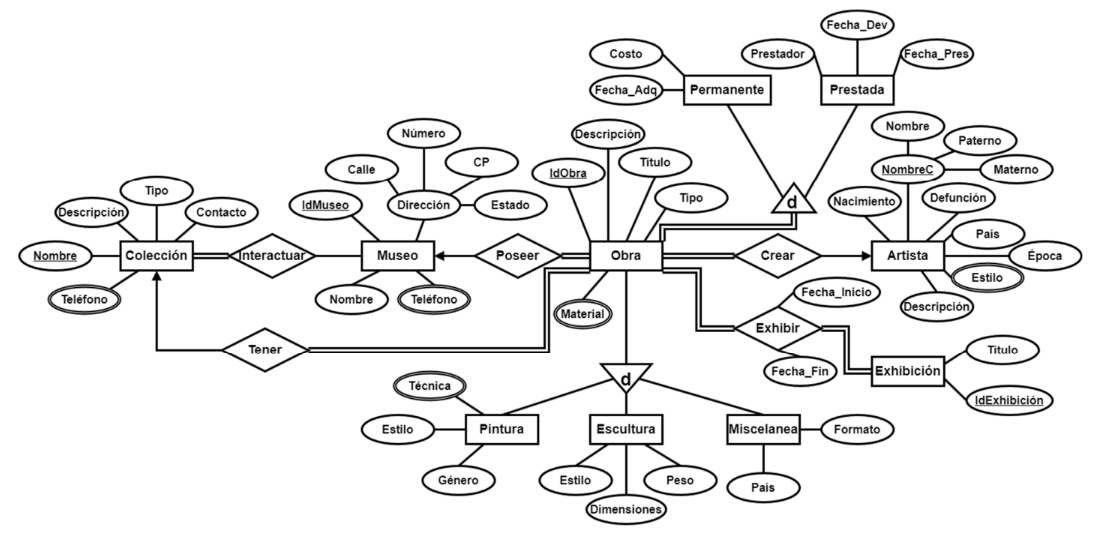
\includegraphics[width=1.1\textwidth]{imagenes/Diagrama(2a)E-R.png}
    \label{fig:mi_imagen}
\end{figure}

\textbf{Entidades fuertes:}\\
\begin{enumerate}
    \item Colección(\underline{NombreColección}, Descripción, Tipo, Contacto)
    \item TeléfonoColección(\underline{Nombre}, \underline{Teléfono})
    \item Museo(\underline{IdMuseo}, Calle, Número, CP, Estado, Nombre)
    \item TelefónoMuseo(\underline{IdMuseo}, \underline{Teléfono})
    \item Exhibición(\underline{IdExhibición}, Título)
    \item Artísta(\underline{Nombre}, \underline{Materno}, \underline{Paterno}, Nacimiento, Defunción, País, Época, Descripción)
    \item Estilo(\underline{Nombre}, \underline{Materno}, \underline{Paterno}, \underline{Estilo})
    \item Obra(\underline{IdObra}, \dotuline{NombreColección}, \dotuline{IdMuseo}, Descripción, Título,Tipo)
    \item MaterialObra(\underline{IdObra}, \underline{Material})
    \item Pintura(\underline{IdObra}, Estilo, Género)
    \item TécnicaPintura(\underline{IdObra}, \underline{Técnica})
    \item Escultura(\underline{IdObra}, Estilo, Dimensiones, Peso)
    \item Miscelanea(\underline{IdObra}, Formato, País)
    \item Permanente(\underline{IdObra}, Fecha-Adq, Costo)
    \item Prestada(\underline{IdObra}, Prestador, Fecha-Dev, Fecha-Pres)
\end{enumerate}
\textbf{Relaciones fuertes}\\
\begin{enumerate}
    \item Interactuar(\dotuline{NombreColección}, \dotuline{IdMuseo})
    \item Exhibir(\dotuline{IdObra}, \dotuline{IdExhibición}, Fecha-inicio, Fecha-Fin)
    \item Crear(\dotuline{IdObra}, \dotuline{Nombre}, \dotuline{Materno}, \dotuline{Paterno})
\end{enumerate}
\textbf{Consideraciones}
\begin{enumerate}
    \item \textbf{Especialización Parcial (Pintura, Escultura, Miscelanea):}\\
    Es parcial y disjunta porque una obra solo puede ser de un tipo a la vez, y además es opcional, ya que pueden existir obras en el catálogo general que no entren estrictamente en ninguna de estas tres categorías. Por esta razón, la tabla Obra conserva todos los datos generales (como \texttt{IdObra}, \texttt{Título}, \texttt{Descripción}) y cada subtabla almacena únicamente los atributos específicos de su categoría.

    \item \textbf{Especialización Total (Permanente y Prestada):}\\
    Es total y disjunta porque toda obra debe ser obligatoriamente permanente o prestada, sin poder e pertenecer a ambas categorías al mismo tiempo. Para evitar duplicar información de forma innecesaria, se mantuvieron las tablas Permanente y Prestada cada una con sus datos correspondientes pero la información general se concentra únicamente en Obra.
\end{enumerate}

\begin{figure}[htbp]
    \centering
    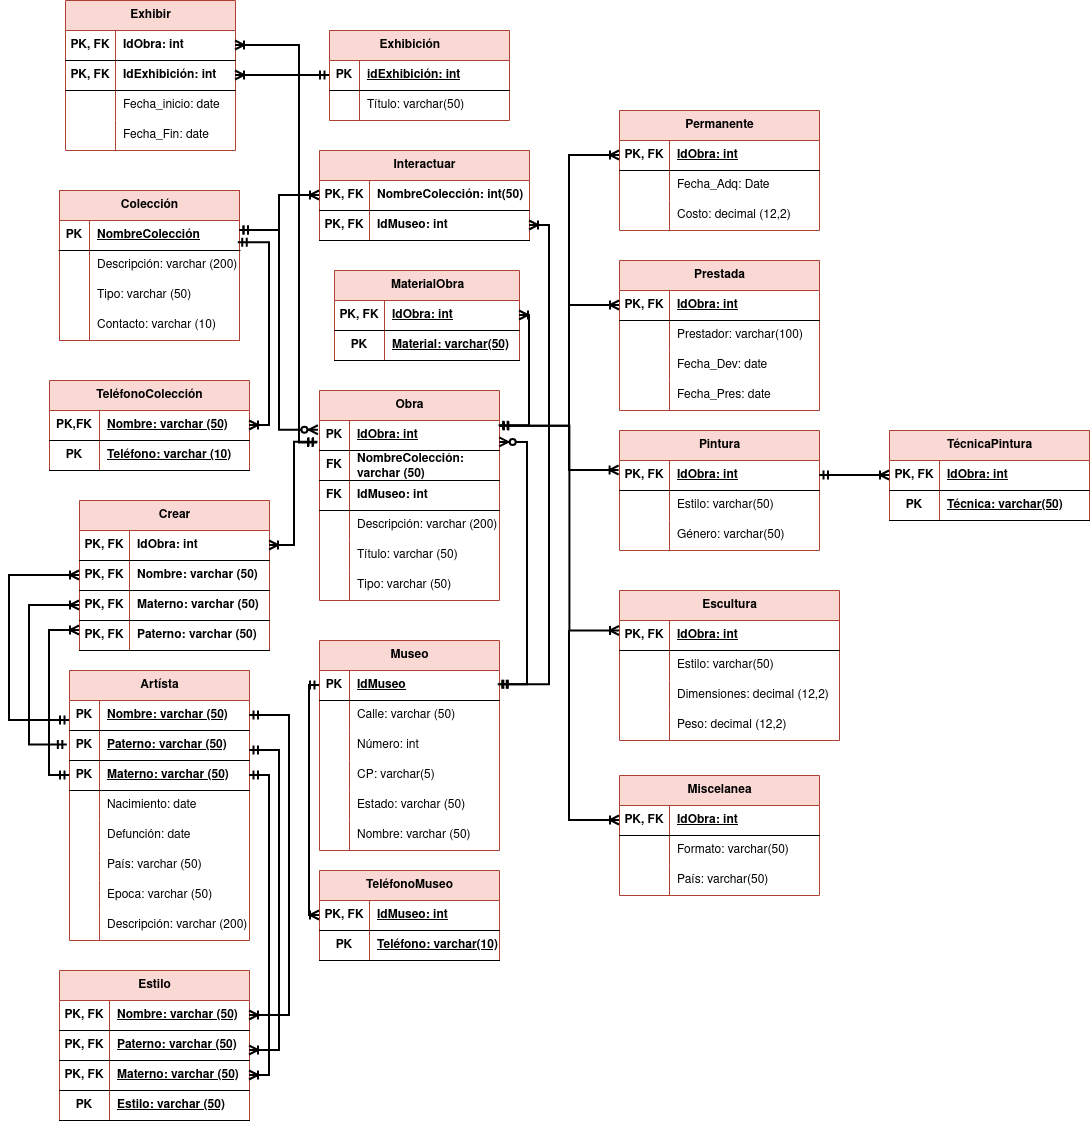
\includegraphics[width=1.1\textwidth]{imagenes/Diagrama2AR.drawio.png}
    \label{fig:mi_imagen}
\end{figure}

 

No se realizaron modificaciones al diseño E-R original; el diagrama se conserva tal cual. Las decisiones tomadas durante la traducción se detallan a continuación.\\ \\

\subsection*{Modelo Entidad-Relación}

\begin{figure}[H]
  \centering
 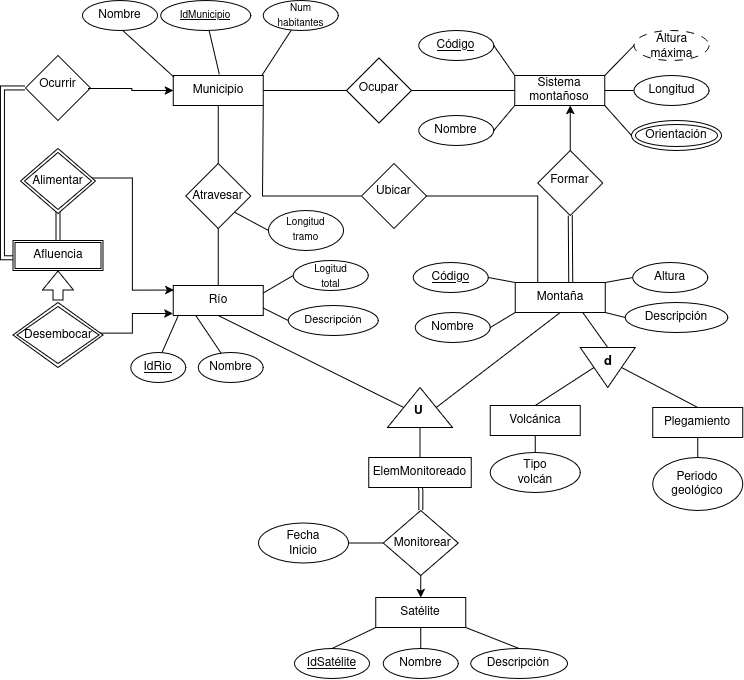
\includegraphics[width=\textwidth]{imagenes/Ejercicio2b(E-R).png}
  \caption{Modelo E-R del Sistema de Información Geográfica}
\end{figure}

\begin{figure}[H]
  \centering
 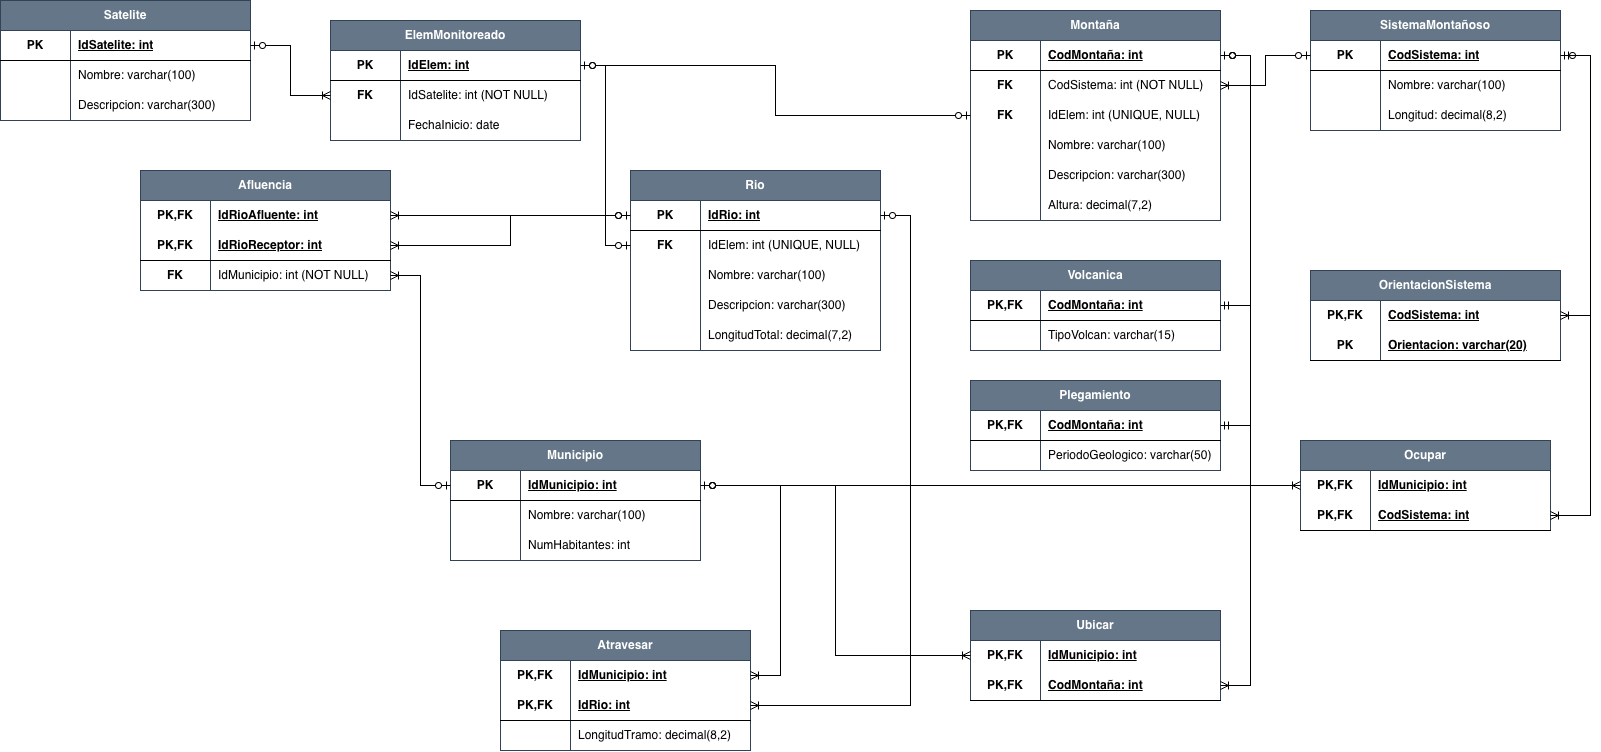
\includegraphics[width=\textwidth]{imagenes/Ejercicio2b(Relacional).png}
  \caption{Traducción al Modelo Relacional del Sistema de Información Geográfica}
\end{figure}

\subsection*{Traducción al Modelo Relacional}
\noindent
Los atributos de la llave primaria aparecen \pk{subrayados} y las llaves foráneas se marcan con el superíndice \textsuperscript{FK}.\\ \\
\textbf{Satelite}(\pk{IdSatelite},\ Nombre,\ Descripcion)\\ \\
\textbf{ElemMonitoreado}(\pk{IdElem},\ \fk{IdSatelite},\ FechaInicio)\\ \\
\textbf{Rio}(\pk{IdRio},\ \fk{IdElem},\ Nombre,\ Descripcion,\ LongitudTotal)\\ \\
\textbf{SistemaMontañoso}(\pk{CodSistema},\ Nombre,\ Longitud)\\ \\
\textbf{OrientacionSistema}(\pkfk{CodSistema},\ \pk{Orientacion})\\ \\
\textbf{Montaña}(\pk{CodMontaña},\ \fk{CodSistema},\ \fk{IdElem},\ Nombre,\ Descripcion,\ Altura)\\ \\
\textbf{Volcanica}(\pkfk{CodMontaña},\ TipoVolcan)\\ \\
\textbf{Plegamiento}(\pkfk{CodMontaña},\ PeriodoGeologico)\\ \\
\textbf{Municipio}(\pk{IdMunicipio},\ Nombre,\ NumHabitantes)\\ \\
\textbf{Atravesar}(\pkfk{IdMunicipio},\ \pkfk{IdRio},\ LongitudTramo)\\ \\
\textbf{Ubicar}(\pkfk{IdMunicipio},\ \pkfk{CodMontaña})\\ \\
\textbf{Ocupar}(\pkfk{IdMunicipio},\ \pkfk{CodSistema})\\ \\
\textbf{Afluencia}(\pkfk{IdRioAfluente},\ \pkfk{IdRioReceptor},\ \fk{IdMunicipio})


\subsection*{Restricciones de entidad}

\subsubsection*{Satelite}

\begin{longtable}{p{2.2cm} p{2.2cm} p{5.8cm} p{4.2cm} p{1.5cm}}
\toprule
\textbf{Atributo} & \textbf{Tipo} & \textbf{Dominio} & \textbf{Restricciones} & \textbf{Llave} \\
\midrule
\endfirsthead

\toprule
\textbf{Atributo} & \textbf{Tipo} & \textbf{Dominio} & \textbf{Restricciones} & \textbf{Llave} \\
\midrule
\endhead

\bottomrule
\endfoot


IdSatelite
& int
& Números mayores a 0
& NOT NULL (autoincremental)
& PK \\

Nombre
& varchar(100)
& Cadenas de hasta 100 caracteres.
& NOT NULL
&  \\

Descripcion
& varchar(300)
& Cadenas de hasta 300 caracteres.
& NULL permitido
&  \\

\end{longtable}


\subsubsection*{ElemMonitoreado}

\begin{longtable}{p{2.2cm} p{2.2cm} p{5.8cm} p{4.2cm} p{1.5cm}}
\toprule
\textbf{Atributo} & \textbf{Tipo} & \textbf{Dominio} & \textbf{Restricciones} & \textbf{Llave} \\
\midrule
\endfirsthead

\toprule
\textbf{Atributo} & \textbf{Tipo} & \textbf{Dominio} & \textbf{Restricciones} & \textbf{Llave} \\
\midrule
\endhead

\bottomrule
\endfoot


IdElem
& int
& Números mayores a 0
& NOT NULL (autoincremental)
& PK \\

IdSatelite
& int
& Números mayores a 0
& NOT NULL
& FK \\

FechaInicio
& date
& Fechas válidas con formato AAAA-MM-DD.
& NOT NULL
&  \\

\end{longtable}


\subsubsection*{Rio}

\begin{longtable}{p{2.6cm} p{2.2cm} p{5.8cm} p{4.2cm} p{1.5cm}}
\toprule
\textbf{Atributo} & \textbf{Tipo} & \textbf{Dominio} & \textbf{Restricciones} & \textbf{Llave} \\
\midrule
\endfirsthead

\toprule
\textbf{Atributo} & \textbf{Tipo} & \textbf{Dominio} & \textbf{Restricciones} & \textbf{Llave} \\
\midrule
\endhead

\bottomrule
\endfoot


IdRio
& int
& Números mayores a 0
& NOT NULL (autoincremental)
& PK \\

IdElem
& int
& Números mayores a 0
& NULL permitido;

UNIQUE
& FK \\

Nombre
& varchar(100)
& Cadenas de hasta 100 caracteres.
& NOT NULL
&  \\

Descripcion
& varchar(300)
& Cadenas de hasta 300 caracteres.
& NULL permitido
&  \\

LongitudTotal
& decimal(7,2)
& Números decimales mayores a 0
& NOT NULL;

Revisar: (LongitudTotal $>$ 0)
&  \\

\end{longtable}


\subsubsection*{SistemaMontañoso}

\begin{longtable}{p{2.2cm} p{2.2cm} p{5.8cm} p{4.2cm} p{1.5cm}}
\toprule
\textbf{Atributo} & \textbf{Tipo} & \textbf{Dominio} & \textbf{Restricciones} & \textbf{Llave} \\
\midrule
\endfirsthead

\toprule
\textbf{Atributo} & \textbf{Tipo} & \textbf{Dominio} & \textbf{Restricciones} & \textbf{Llave} \\
\midrule
\endhead

\bottomrule
\endfoot


CodSistema
& int
& Números mayores a 0
& NOT NULL (autoincremental)
& PK \\

Nombre
& varchar(100)
& Cadenas de hasta 100 caracteres.
& NOT NULL
&  \\

Longitud
& decimal(8,2)
& Números decimales mayores a 0
& NOT NULL;

Revisar: (Longitud $>$ 0)
&  \\

\end{longtable}


\subsubsection*{OrientacionSistema}

\begin{longtable}{p{2.2cm} p{2.2cm} p{5.8cm} p{4.2cm} p{1.5cm}}
\toprule
\textbf{Atributo} & \textbf{Tipo} & \textbf{Dominio} & \textbf{Restricciones} & \textbf{Llave} \\
\midrule
\endfirsthead

\toprule
\textbf{Atributo} & \textbf{Tipo} & \textbf{Dominio} & \textbf{Restricciones} & \textbf{Llave} \\
\midrule
\endhead

\bottomrule
\endfoot


CodSistema
& int
& Números mayores a 0
& NOT NULL
& PK, FK \\

Orientacion
& varchar(20)
& Cadenas dentro de la lista (Norte, Sur, Este, Oeste)
& NOT NULL;

Revisar que el valor sea uno en (Norte, Sur, Este, Oeste)
& PK \\

\end{longtable}


\subsubsection*{Montaña}

\begin{longtable}{p{2.2cm} p{2.2cm} p{5.8cm} p{4.2cm} p{1.5cm}}
\toprule
\textbf{Atributo} & \textbf{Tipo} & \textbf{Dominio} & \textbf{Restricciones} & \textbf{Llave} \\
\midrule
\endfirsthead

\toprule
\textbf{Atributo} & \textbf{Tipo} & \textbf{Dominio} & \textbf{Restricciones} & \textbf{Llave} \\
\midrule
\endhead

\bottomrule
\endfoot


CodMontaña
& int
& Números mayores a 0
& NOT NULL (autoincremental)
& PK \\

CodSistema
& int
& Números mayores a 0
& NOT NULL
& FK \\

IdElem
& int
& Números mayores a 0
& NULL permitido;

UNIQUE
& FK \\

Nombre
& varchar(100)
& Cadenas de hasta 100 caracteres.
& NOT NULL
&  \\

Descripcion
& varchar(300)
& Cadenas de hasta 300 caracteres.
& NULL permitido
&  \\

Altura
& decimal(7,2)
& Números decimales mayores a 0
& NOT NULL;

Revisar: (Altura $>$ 0)
&  \\

\end{longtable}


\subsubsection*{Volcanica}

\begin{longtable}{p{2.2cm} p{2.2cm} p{5.8cm} p{4.2cm} p{1.5cm}}
\toprule
\textbf{Atributo} & \textbf{Tipo} & \textbf{Dominio} & \textbf{Restricciones} & \textbf{Llave} \\
\midrule
\endfirsthead

\toprule
\textbf{Atributo} & \textbf{Tipo} & \textbf{Dominio} & \textbf{Restricciones} & \textbf{Llave} \\
\midrule
\endhead

\bottomrule
\endfoot

CodMontaña
& int
& Números mayores a 0
& NOT NULL
& PK, FK \\

TipoVolcan
& varchar(15)
& Cadenas de hasta 15 caracteres.
& NOT NULL
&  \\

\end{longtable}


\subsubsection*{Plegamiento}

\begin{longtable}{p{3.2cm} p{2.2cm} p{5.3cm} p{4.0cm} p{1.7cm}}
\toprule
\textbf{Atributo} & \textbf{Tipo} & \textbf{Dominio} & \textbf{Restricciones} & \textbf{Llave} \\
\midrule
\endfirsthead

\toprule
\textbf{Atributo} & \textbf{Tipo} & \textbf{Dominio} & \textbf{Restricciones} & \textbf{Llave} \\
\midrule
\endhead

\bottomrule
\endfoot


CodMontaña
& int
& Números mayores a 0
& NOT NULL
& PK, FK \\

PeriodoGeologico
& varchar(50)
& Cadenas de hasta 50 caracteres.
& NOT NULL
&  \\

\end{longtable}


\subsubsection*{Municipio}

\begin{longtable}{p{2.7cm} p{2.2cm} p{4.8cm} p{4.2cm} p{1.5cm}}
\toprule
\textbf{Atributo} & \textbf{Tipo} & \textbf{Dominio} & \textbf{Restricciones} & \textbf{Llave} \\
\midrule
\endfirsthead

\toprule
\textbf{Atributo} & \textbf{Tipo} & \textbf{Dominio} & \textbf{Restricciones} & \textbf{Llave} \\
\midrule
\endhead

\bottomrule
\endfoot


IdMunicipio
& int
& Números mayores a 0
& NOT NULL (autoincremental)
& PK \\

Nombre
& varchar(100)
& Cadenas de hasta 100 caracteres.
& NOT NULL
&  \\

NumHabitantes
& int
& Números enteros mayores o iguales a 0
& NOT NULL;

Revisar: (NumHabitantes $\geq$ 0)
&  \\

\end{longtable}


\subsubsection*{Atravesar}

\begin{longtable}{p{2.6cm} p{2.2cm} p{5.8cm} p{4.2cm} p{1.5cm}}
\toprule
\textbf{Atributo} & \textbf{Tipo} & \textbf{Dominio} & \textbf{Restricciones} & \textbf{Llave} \\
\midrule
\endfirsthead

\toprule
\textbf{Atributo} & \textbf{Tipo} & \textbf{Dominio} & \textbf{Restricciones} & \textbf{Llave} \\
\midrule
\endhead

\bottomrule
\endfoot


IdMunicipio
& int
& Números mayores a 0
& NOT NULL
& PK, FK \\

IdRio
& int
& Números mayores a 0
& NOT NULL
& PK, FK \\

LongitudTramo
& decimal(8,2)
& Números decimales mayores a 0
& NOT NULL;

Revisar: (LongitudTramo $>$ 0)
&  \\

\end{longtable}


\subsubsection*{Ubicar}

\begin{longtable}{p{2.2cm} p{2.2cm} p{5.8cm} p{4.2cm} p{1.5cm}}
\toprule
\textbf{Atributo} & \textbf{Tipo} & \textbf{Dominio} & \textbf{Restricciones} & \textbf{Llave} \\
\midrule
\endfirsthead

\toprule
\textbf{Atributo} & \textbf{Tipo} & \textbf{Dominio} & \textbf{Restricciones} & \textbf{Llave} \\
\midrule
\endhead

\bottomrule
\endfoot

IdMunicipio
& int
& Números mayores a 0
& NOT NULL
& PK, FK \\

CodMontaña
& int
& Números mayores a 0
& NOT NULL
& PK, FK \\

\end{longtable}


\subsubsection*{Ocupar}

\begin{longtable}{p{2.2cm} p{2.2cm} p{5.8cm} p{4.2cm} p{1.5cm}}
\toprule
\textbf{Atributo} & \textbf{Tipo} & \textbf{Dominio} & \textbf{Restricciones} & \textbf{Llave} \\
\midrule
\endfirsthead

\toprule
\textbf{Atributo} & \textbf{Tipo} & \textbf{Dominio} & \textbf{Restricciones} & \textbf{Llave} \\
\midrule
\endhead

\bottomrule
\endfoot


IdMunicipio
& int
& Números mayores a 0
& NOT NULL
& PK, FK \\

CodSistema
& int
& Números mayores a 0
& NOT NULL
& PK, FK \\

\end{longtable}


\subsubsection*{Afluencia}

\begin{longtable}{p{2.5cm} p{2.2cm} p{4.5cm} p{5.7cm} p{1.5cm}}
\toprule
\textbf{Atributo} & \textbf{Tipo} & \textbf{Dominio} & \textbf{Restricciones} & \textbf{Llave} \\
\midrule
\endfirsthead

\toprule
\textbf{Atributo} & \textbf{Tipo} & \textbf{Dominio} & \textbf{Restricciones} & \textbf{Llave} \\
\midrule
\endhead

\bottomrule
\endfoot


IdRioAfluente
& int
& Números mayores a 0
& NOT NULL
& PK, FK \\

IdRioReceptor
& int
& Números mayores a 0
& NOT NULL;

Revisar: (IdRioAfluente $\neq$ IdRioReceptor)
& PK, FK \\

IdMunicipio
& int
& Números mayores a 0
& NOT NULL
& FK \\

\end{longtable}
 \section*{3. Modelo relacional e inserción de tuplas.}

\addcontentsline{toc}{section}{3. Modelo relacional e inserción de tuplas.}

Considera el siguiente \textbf{Modelo E/R}:

\begin{figure}[h!]
    \centering
    
     \includegraphics[width=0.7\textwidth]{imagenes/3.png}

    
\end{figure}

\addcontentsline{toc}{subsection}{a.}

\begin{enumerate}[label=\textbf{\alph*.}]
    \item Completa la tabla que se presenta a continuación, convirtiendo el Modelo E-R en un Modelo Relacional, para todas las opciones de cardinalidad (considera en todos los casos, participación parcial). Indica las relaciones resultantes, su llave primaria y la integridad referencial. Traduce los atributos de izquierda a derecha y considera el formato de traducción: Tabla(llavePk1, llavePk2, \dots, atr1, atr2, \dots, llaveFk1, \dots)

    \vspace{0.5cm}
    \begin{table}[h!]
        \centering
        \renewcommand{\arraystretch}{2.5} 
        \begin{tabular}{|c|p{12cm}|}
            \hline
            \textbf{Modelo E-R} & \textbf{Modelo Relacional} \\
            \hline
            $\mathbf{M : N}$ &  A(\underline{llavePKa1},
                                  \underline{llavePKa2}, 
                                  a3)
                                  
                                B(\underline{llavePKb},
                                  b1)

                                ab(\underline{llaveFKa1},
                                   \underline{llaveFKa2},
                                   \underline{llaveFKb},
                                   ab1)\\
            \hline
            $\mathbf{1 : N}$ &  A(\underline{llavePKa1},
                                  \underline{llavePKa2},            
                                  a3)
                                  
                                B(\underline{llavePKb},
                                  b1,
                                  ab1,
                                  llaveFKa1,
                                  llaveFKa2)\\
            \hline
            $\mathbf{N : 1}$ &  A(\underline{llavePKa1},
                                  \underline{llavePKa2},
                                  a3,
                                  ab1,
                                  llaveFKb)
                                  
                                B(\underline{llavePKb},
                                  b1)\\
            \hline
            $\mathbf{1 : 1}$ &  A(\underline{llavePKa1},
                                  \underline{llavePKa2}, 
                                  a3)
                                  
                                B(\underline{llavePKb},
                                  b1)

                                ab(\underline{llaveFKa1},
                                   \underline{llaveFKa2},
                                   \underline{llaveFKb},
                                   ab1)\\
            \hline
        \end{tabular}
    \end{table}
    \vspace{0.5cm}
    \newpage

    \addcontentsline{toc}{subsection}{b.}
    \item Del inciso a) toma el MR que obtuviste para la cardinalidad M : N. Asume que los atributos a1, b y ab1 son de tipo entero, mientras que a2, a3 y b1 son de tipo cadena. Supón que la relación A tiene 4 tuplas con los siguientes valores (2,'ww','a'), (4,'xx','b'), (6,'yy','c'), (8,'zz','d') y la relación B tiene 5 tuplas identificadas por los valores 17, 27, 37, 47, 57. Los incisos que se presentan a continuación representan un conjunto de tuplas a insertar (en ese orden) en la relación AB, indica cuál conjunto se puede insertar completamente en dicha relación. Justifica tu respuesta en cada caso. En caso de no ser posible, indica un conjunto de 5 tuplas que si se puedan insertar.

\begin{enumerate}[label=\roman*.]
    \item (8,'zz', 17, 5); (6,'yy', 57, 10); (4,'xx', 27, 15); (2,'ww', 37, 20); (4,'xx', 27, 15)
    
    En este caso, notemos que la tupla 3 y 5 son iguales, de modo que al tratar de insertar la última tupla, los valores de las llaves se repetirán y se marcará un error por duplicado de llaves. Para solucionarlo, basta con modificar el valor de 27 en la última tupla por cualquier otro disponible, como 17. De este modo, una tupla válida sería la siguiente:
    \begin{itemize}
        \item (8,'zz', 17, 5); (6,'yy', 57, 10); (4,'xx', 27, 15); (2,'ww', 37, 20); (4,'xx', 17, 15)
    \end{itemize}
    
    \item (17,'zz', 2,'m'); (27,'yy', 4,'n'); (37,'xx', 6,'o'); (47,'ww', 8,'p'); (57,'zz', 4,'q')
    
      Por una parte, notemos que los atributos de las inserciones están desordenados. Al traducir la relación al modelo relacional usando la indicación de agrupar los atributos de izquierda a derecha, el orden debería ser: ab(\underline{llaveFKa1}, \underline{llaveFKa2}, \underline{llaveFKb}, ab1), sin embargo, parece tener el orden: ab(llaveFKb, llaveFKa2, llaveFKa1, ab1). De este modo, un primer error está en cuestión de integridad referencial, pues no podemos encontrar las llaves 17, 27, 37, 47 y 57 en la tabla de A, y de la misma forma, no podemos encontrar los números 2, 4, 6 y 8 en la tabla de B. Por otro lado, siguiendo el orden en el que se escriben los atributos, el último elemento es el atributo ab1, que se menciona que es un entero, mientras que en las inserciones es una cadena, por lo que existe un error sobre el tipo de dato usado. Una tupla válida sería:
    \begin{itemize}       
        \item (2,'ww', 17, 1); (4,'xx', 27, 3); (6,'yy', 37, 5); (8,'zz', 47, 7); (4,'xx', 57, 9)   
    \end{itemize}

    
    \item (2,'a', 17, 23); (4,'b', 27, 24); (6,'c', 37, 25); (8,'d', 47, 26); (2,'a', 57, 27)
    
    Siguiendo el orden en que se escriben los atributos en la tabla anterior, notemos que los primeros dos elementos deben coincidir con llaves primarias existentes en la tabla correspondiente a la entidad A; particularmente, el segundo elemento debería ser el par correspondiente al primer elemento de la tupla, sin embargo, este segundo elemento no está en el conjunto de posibles valores que puede tomar a2. De este modo, al tratar de insertar la tupla tendremos un error de integridad referencial. Una tupla correcta sería:
    \begin{itemize}
        \item (2,'ww', 17, 23); (4,'xx', 27, 24); (6,'yy', 37, 25); (8,'zz', 47, 26); (2,'ww', 57, 27)
    \end{itemize}
    
    \item (2,'ww', 57, 2); (4,'xx', 37, 4); (6,'yy', 17, 6); (8,'zz', 37, 8); (4,'xx', 47, 10)

    Esta tupla es totalmente correcta. Notemos que, siguiendo el orden de los atributos en la tabla anterior, los primeros dos elementos corresponden a un par válido en la tabla de A, el siguiente elemento también es un valor válido en la tabla de B, y el último elemento es un número, cumpliendo con el tipo de dato correspondiente al atributo ab1. Además, ninguna tupla se repite.
\end{enumerate}

    \addcontentsline{toc}{subsection}{c.}
    \item Del inciso a) toma como base el MR que obtuviste para la cardinalidad 1:N. Los incisos que se presentan a continuación representan un conjunto de tuplas a insertar (en ese orden) en la relación B, indica cuál conjunto se puede insertar completamente en dicha relación. Justifica tu respuesta en cada caso. En caso de no ser posible, indica un conjunto de 5 tuplas que sí se puedan insertar.

    Tomemos, al igual que en los demás incisos, el contexto proporcionado en el inciso b) para las llaves de A y B.
    \begin{enumerate}[label=\roman*.]
     \item (2,'f',57,'zz',10); (4,'g',47,'yy',15); (6,'h',37,'xx',10); (8,'i',27,'ww',15); (2,'j',17,'yy',20)
    
     Notemos que estas 5 tuplas no serán aceptadas pues el orden de la tupla es incorrecto. El orden correcto (solo agregando el tipo de dato para cada elemento) es el siguiente: (int, varchar, int, int, varchar) como se vio en la fila del 1:N de la tabla del inciso a), mientras que en las 5 tuplas tenemos un varchar en la posición 4 (de izquierda a derecha) en lugar de un int.

     Por lo que propongo el siguiente conjunto de 5 tuplas que lo satisface, corrigiendo los errores de orden y preservando la integridad referencial:
     
     (57,'f',10,8,'zz'); (47,'g',15,6,'yy'); (37,'h',10,4,'xx'); (27,'i',15,2,'ww'); (17,'j',20,6,'yy')

    \vspace{.5cm}
    \item (57,8,'zz','f',2); (47,6,'yy','g',4); (37,4,'xx','h',6); (27,2,'ww','i',8); (17,6,'yy','j',6)
    
    Similarmente al inciso pasado, el orden de la tupla es INCORRECTO, por lo que estas 5 tuplas tampoco serán aceptadas; particularmente la posición dos de la tupla tiene un int en vez de tener una cadena. Podemos ordenar los elementos de las tuplas con el formato correcto proporcionado en la tabla del inciso a), donde se nota que así se preservaría el orden, la integridad referencial y la propiedad de relación 1:N (por lo que se permite que el par 6,'yy' se utilice para dos valores de la llave de B):

    (57,'f',2,8,'zz'); (47,'g',4,6,'yy'); (37,'h',6,4,'xx'); (27,'i',8,2,'ww'); (17,'j',6,6,'yy')

    \vspace{.5cm}
    \item (17,'f',8,'zz',1); (27,'g',6,'yy',2); (37,'h',4,'xx',3); (27,'i',2,'ww',4); (17,'j',6,'yy',5)

    Este conjunto sigue el orden del conjunto I, es decir, un orden incorrecto donde las llaves foráneas de A están en medio en lugar de en el extremo derecho. Ordenando correctamente notamos que las tuplas respetan la integridad referencial y además la relación 1:N (por ello es válido que las llaves 6,'yy' de A se repitan para dos valores de B); la única corrección adicional necesaria es elegir valores únicos para la llave primaria de B (ya que 17 y 27 se repetían), por lo que queda como:

    (17,'f',1,8,'zz'); (27,'g',2,6,'yy'); (37,'h',3,4,'xx'); (47,'i',4,2,'ww'); (57,'j',5,6,'yy')

    \vspace{.5cm}
    \item  (37,'f',8,2,'ww'); (47,'g',6,4,'xx'); (27,'h',4,6,'yy'); (17,'i',2,8,'zz'); (57,'j',6,4,'xx')

    Finalmente, se puede notar que en efecto este conjunto de tuplas es aceptado, respeta la integridad referencial usando las llaves de A y la llave de B definidas previamente y, además, en el orden correcto. Finalmente, las dos posiciones restantes cumplen efectivamente con los tipos en sus posiciones correctas, por lo que este conjunto es insertado exitosamente.
     \end{enumerate}

     \addcontentsline{toc}{subsection}{d.}
    \item Considera el mismo escenario del inciso b) para las relaciones A y B. Toma como base el Modelo Relacional que obtuviste para la cardinalidad 1:1. Supón que tu modelo tiene participación parcial de ambos lados. Propón un conjunto de 5 tuplas que se pueda insertar en la relación ab y un conjunto que no se pueda insertar (también de 5 tuplas). Justifica tu respuesta en cada caso.
    \begin{enumerate}[label=\roman*.]
        \item Primero veamos qué tuplas se podrían aceptar y por qué. Cabe destacar que, dado que la entidad A solo cuenta con 4 tuplas en el inciso b), \textbf{es imposible proponer 5 tuplas válidas} sin antes agregar nuevos registros a la tabla A, esto por la restricción de cardinalidad 1:1, por lo que cada par de llaves de A solo se puede realcionar con una de B. Por ello, proponemos las unicas 4 posibles:

         (2,'ww',17,5); (4,'xx',27,10); (6,'yy',37,15); (8,'zz',47,20)

         Así que notemos que satisfacen todas las condiciones para que sean insertadas, las dividiré en 3:
         \begin{enumerate}
             \item Preservan la integridad referencial: Esto es, los dos primeros términos de la tupla corresponden a las llaves foráneas de la entidad A, y las siguientes posiciones a la llave foránea de la entidad B, donde efectivamente las 4 tuplas satisfacen que corresponden a las llaves ya existentes predefinidas en el inciso b).
             \item Correcto el tipo de dato: Todos los elementos de las 4 tuplas satisfacen seguir los tipos de datos definidos en el inciso b): (int, cadena, int, int) por lo que cumplen este punto.
             \item Restricción 1:1: Al ser una relación uno a uno, las llaves de A se pueden relacionar solo con una llave de B y viceversa. Las 4 tuplas respetan esto, ya que ninguna llave de A ni de B se repite. Por esta misma regla es imposible insertar una quinta tupla usando las llaves existentes.
         \end{enumerate}

         \item Ahora veamos 5 que NO son aceptadas y por qué:

        (2,'ww',17,5); (4,'xx',27,'zz'); (5,'yy',37,15); (1,'ww','zz',25.5); (2,'ww',57,25)

        Notemos que cada tupla incumple al menos uno de los requerimientos del punto pasado:
        \begin{enumerate}
            \item (2,'ww',17,5): Aunque las llaves existen en las entidades originales, esta tupla viola la restricción de cardinalidad uno a uno, pues la llave de A (2,'ww') ya fue relacionada previamente con otra llave de B, y no se puede relacionar con más de una.
            \item (4,'xx',27,'zz'): Aunque la integridad referencial se satisface en parte y no está repetida, el último elemento NO corresponde con el tipo de dato correcto (debería ser int).
            \item (5,'yy',37,15): La integridad referencial es violada por el primer elemento pues la entidad A NO tiene la llave compuesta 5, 'yy'. Por lo que no acepta la tupla.
            \item (1,'ww','zz',25.5): Esta tupla no respeta la integridad referencial ni los tipos de datos en la llave de B, por lo que no sería aceptada.
            \item (2,'ww',57,25): Misma razón que en el punto 1).
        \end{enumerate}
     \end{enumerate}
\end{enumerate} 

 \section*{4.}
\subsection*{a.}
Es posible que dos departamentos tengan el nombre \textit{`Sistemas'} pues, como no son parte de la llave primaria (PK) del tipo de entidad, entonces no tiene restricciones de unicidad explícitas, por lo que la afirmación es verdadera.

\subsection*{b.}
Dada la estructura de la tabla de relación de \texttt{Trabajar}, cuya PK se compone de 1 entidad de \texttt{Empleado} y 1 de \texttt{Departamento}, entonces la restricción solamente indica que no se puede repetir una relación de trabajo entre los mismos valores de identificador de \texttt{Empleado}, de identificador de \texttt{Departamento} y del atributo \texttt{desde}, por lo que, si dos entidades de tipo \texttt{Empleado} son distintas, entonces sí se pueden relacionar con la misma entidad \texttt{Departamento}, por lo que la afirmación es verdadera.

\subsection*{c.}
Para las tablas de relación de \texttt{Trabajar} o de \texttt{Administrar}, el que haya identificadores de \texttt{Empleado} o de \texttt{Departamento} registrados en una fila de una de las tablas no genera restricciones en la otra a nivel lógico, ya que éstas no tienen relación entre sí, por lo que, como ambas tablas \texttt{Trabajar} y \texttt{Administrar} pueden tener filas con los mismos identificadores, entonces un empleado puede trabajar en un departamento y administrar otro a la vez, por lo que la afirmación es verdadera.

\subsection*{d.}
Como se explicó en el inciso anterior, \texttt{Trabajar} o de \texttt{Administrar} no tienen restricciones entre sí en cuanto a los valores que se pueden o deben almacenar por lo que, como un \texttt{Empleado} puede trabajar en un \texttt{Departamento} y administrar otro a la vez, entonces no requiere trabajar en el \texttt{Departamento} que administra para cumplir con las restricciones, por lo que la afirmación es falsa.

\subsection*{e.}
Ya que la PK de \texttt{Trabajar} determina que la tupla que la compone debe ser única, entonces en esta relación no se pueden repetir a la vez los tres valores \texttt{NúmEmpleado}, \texttt{NúmDepto} \texttt{Desde}. No obstante, esto no se restringe a la repetición de hasta dos valores (pues la PK sigue siendo identificable a partir de los diferentes valores del registro de lque no se repite), entonces se pueden repetir los valores de \texttt{NúmEmpleado} y \texttt{Desde} en una fila si se cambian los valores de \texttt{NúmDepto} i.e. un empleado puede trabajar en dos departamentos diferentes a partir de la misma fecha, por lo que la afirmación es verdadera.

\subsection*{f.}
Ya que puede un modelo relacional por si mismo no puede aplicar restricciones entre los atributos de una misma entidad, y que el diagrama no presenta espacificaciones adjuntas, entonces no se tiene una restricción entre \texttt{hasta} y \texttt{desde} que determine que uno debe ser anterior al otro, por lo que la afirmación es falsa.

\subsection*{g.}
Como se mencionó en el inciso $e.$, la relación \texttt{Trabajar} permite repetir valores de la PK siempre y cuando no sean todos. Es por esto que la tabla \texttt{Trabajar} refleja que la relación entre \texttt{NúmEmpleado} y \texttt{NúmDepto} es de cardinalidad $N:M$. Por esto, dado un identificador de empleado $x$, si bien es posible conocer los departamentos en los que trabaja el respectivo empleado mediante la línea de comandos
\begin{center}
    \texttt{SELECT NúmDepartamento FROM Trabajar WHERE NúmEmpleado = x;}
\end{center}
querer conocer exactamente el \textbf{único} \texttt{Departamento} donde éste trabaja no tiene sentido, por lo que la afirmación es falsa.

\subsection*{h.}
Si bien se pueden gestionar correctamente las restricciones entre valores en la implementación del diagrama, como se comentó en el inciso $f.$, el diagrama por sí mismo carece de dichas restricciones, por lo que, ya que la PK de la tabla de \texttt{Salario} se conforma por la dupla de \texttt{NúmEmpleado} y \texttt{Desde}, basta con que el segundo atributo sea distinto entre dos filas para que el empleado se pueda repetir por lo que, si se dan los siguientes condiciones en $Salario$, entonces un mismo empleado sí puede tener asignado más de un salario, por lo que la afirmación del inciso es falsa:
\begin{enumerate}
    \item La fecha de inicio no se repite pero el identificador de empleado sí en dos filas (asignación de salario al mismo empleado).
    \item El salario es distinto entre ambas filas (asignación de salarios distintos al empleado).
    \item Las fechas de \texttt{hasta} son posteriores a sus respectivas fechas de \texttt{desde} (se da intervalo real), y al menos un día se encuentra en ambos intervalos a la vez (los dos periodos de salario se dan a la vez).
\end{enumerate}

\subsection*{i.}
Ya que, por definición, todas las columnas que forman parte de la PK son estrictamente no nulas entonces, por cada registro de \texttt{Salario}, debe haber un identificador de empleado y una fecha de inicio asociados i.e. obligatoriamente debe haber valores para \texttt{NúmEmpleado} y \texttt{Desde} asociados, por lo que la proposición del inciso es es falsa.

\subsection*{j.}
Dada la cardinalidad expresada entre \texttt{Administrar} y \texttt{Departamento}, que indica una relación parcial para este último, queda explícito que un \texttt{Departamento} puede ser registrado en la base de datos sin necesidad de tener a alguien encargado de su administración, por lo que la afirmación es falsa.

%\nocite{*} 
%\printbibliography[title={Referencias}]

\end{document}
